% ===== ch05 : 原文 main.tex 第 1055--1300 行（4a 带群作用的 Weinstein 扇区（前半））=====
% 本文件是原文 LaTeX 源码的逐行分片（去掉整段注释掉的旧稿），仅供翻译时对照；最终译文写到 src/chunks/ch05.tex。
\section{Fukaya Categories of Discrete Quotients\label{sec:Fukaya-category-discrete-quotient}}
Suppose $X$ is a Weinstein sector and $G\curvearrowright X$ be a discrete group acting exact symplectically, discrete continuously and freely on $X$. We further assume that the action is \emph{cylindrical}, i.e. in a cylindrical end $\partial_{\infty}X\times [0,+\infty)\hookrightarrow X$ of $X$, the $G$-action on $X$ preserves the cylindrical coordinate $[0,+\infty)$ and is a contactomorphism on each contact boundary at infinity $\partial_{\infty} X$ of $X$.\par
By assumption the quotient space $X/G$ is still a Weinstein sector on $X$ with ideal boundary at infinity $\partial_{\infty} X/G$. In this section, we are going to compute the wrapped Fukaya category $\mathcal{W} (X/G)$ of $X/G$ in terms of the wrapped Fukaya category $\mathcal{W} (X)$. Our main theorem for this section is:
\begin{thm}[Wrapped Fukaya Categories of Quotients]\label{thm:wrapped-Fukaya-quotient}
    There is an equivalence of $A_{\infty}$-categories
% ---- 原文行 1060 ----
    \[
        \mathcal{W} (X/G)\simeq\mathcal{W} (X)/G \simeq\mathcal{W}(X)_G
    \]
    after twisted completion, where $\mathcal{W} (X)/G$ is the $A_{\infty}$-variant of dg orbit categories developed by Fan-Keller-Qiu \cite{FKQ24} and $\mathcal{W}(X)_G$ is the homotopy quotient of $\mathcal{W}(X)$ by the $G$-action, whose equivalence with $\mathcal{W}(X)/G$ was proved by Christ \cite{Christ26}.
\end{thm}
\subsection{Weinstein sectors with group action.} In this section we recall the definition of Weinstein sectors and construct Weinstein structures on Weinstein sectors that is invariant under a finitely generated discrete group action. Recall that
\begin{dfn}\label{defn:Liouville-sector-inf}
    A \emph{Liouville sector} is a triple $(X,\omega,Z)$ where $(X,\omega)$ is a symplectic manifold with boundary and $Z$ is a complete vector field on $X$ such that 
    \begin{enumerate}[\indent (i)]
        \item (Infinite-type) There exists an exhaustion $X=\displaystyle\bigcup_i X_i$ where $X_0\subseteq X_1\subseteq\dotsb$ is a sequence of compact symplectic manifolds with corners, such that $Z$ is outward-pointing along $\partial X_i\setminus\partial X$ for all $i$.
        \item We have $\mathcal{L}_Z\omega =\omega$, i.e. $Z$ scales $\omega$ exponentially.
        \item There exists a smooth function $I\colon\Nbd (\partial X)\to\mathbb{R}$ defined in an open neighbourhood of $\partial X$, a constant $0<\alpha\leq 1$ and a compact subset $K_i\subseteq\partial X\cap (X_i\setminus X_{i-1})$ for each $i$ such that $ZI=\alpha I$ away from $\displaystyle\bigcup_i K_i$ and the hamiltonian vector field $X_I$ is outward-pointing along $\partial X$.
    \end{enumerate}
    We say $X$ is \emph{Weinstein} if there exists a smooth function $\phi\colon X\to\mathbb{R}$ such that $Z$ is gradient-like for $\phi$, $\phi(\partial X_i)=\{r_i\}$ is a sequence of constants diverging to $\infty$, and the restriction of $\phi$ to $I^{-1}(0)$ defines a Weinstein structure for some chosen smooth function $I$.
\end{dfn}
This definition differs from the original one of Ganatra-Pardon-Shende \cite{GPS20} in that we allow Liouville sectors of infinite type, which when $\partial X=\emptyset$ coincides with \cite{CE12}.
\begin{dfn}\label{defn:G-invariant-Weinstein-sector}
    Let $G$ be a Lie group and $(X,Z_X,\omega_X)$ be a Liouville sector. A $G$-action $G\curvearrowright X$ is \emph{exact symplectic} if for all $g\in G$, there exists $f_g\in C^{\infty} (X;\mathbb{R})$, depending smoothly on $G$, such that $g^{\ast}\lambda_X =\lambda_X +df_g$ where the zeroes of $\lambda_X +df_g$ lie in a compact subset of $X$. It's \emph{compactly supported} if for all $g\in G$, there exists a compact subset $K_g\subseteq X$ such that $g$ is identity outside $K_g$.\par
    An exact symplectic $G$-action on $X$ is \emph{Liouville} if $g^{\ast}\lambda_X =\lambda_X$ for all $g\in G$, where $\lambda_X$ is the symplectic dual of $Z_X$. If $X$ is furthermore Weinstein with Weinstein structure $\phi_X$, then we say $G$-action is \emph{Weinstein} if furthermore $g^{\ast}\phi_X =\phi_X$ for all $g\in G$.
\end{dfn}
% ---- 原文行 1080 ----
\begin{lmm}
    Suppose that $X$ is a Weinstein sector with an exact symplectic $G$-action with compact support and $G$ is a finite group, then there exists a Weinstein structure on $X$ such that $G$ is Weinstein.
\end{lmm}
\begin{proof}
    \textbf{Step 1.} In each cases we can assign to each $g\in G$ a smooth function $f_g\in C^{\infty} (X,\mathbb{R})$ so that $g^{\ast}\lambda_X =\lambda_X +df_g$. We look for Liouville $1$-form $\lambda\coloneqq\lambda_X +df$, for some $f\in C^{\infty}(X,\mathbb{R})$ so that $g^{\ast}\lambda =\lambda$ for all $g\in G$. Plugging in $g$ gives \[
        g^{\ast}\lambda -\lambda =d(f_g +f\circ g-f),
    \]and therefore $f$ should satisfy the identity \begin{equation}\label{eq:invariance-condition}
        f_g +f\circ g-f=0
    \end{equation}for all $g\in G$. Note that for $h\in G$, we have the composition \[
        h^{\ast}g^{\ast}\lambda_X =h^{\ast} (\lambda_X +df_g)=\lambda_X +d(f_h +f_g\circ h)=\lambda_X +df_{gh},
    \]the functions $\{f_g\}_{g\in G}$ must satisfy $f_{gh}=f_h +f_g\circ h$ up to a constant shift, which we can arrange so that the strict identity holds in both situations.\par
    \textbf{Step 2.} Suppose that $G$ is finite, then we consider the function \[
        f=\frac{1}{\vert G\vert}\sum_{g\in G} f_g.
    \]It's not difficult to check that equation \eqref{eq:invariance-condition} holds for any $g\in G$, and therefore the $1$-form $\lambda_G\coloneqq\lambda_X +df$ satisfies $d\lambda_G =\omega_X$ and $g^{\ast}\lambda_G =\lambda_G$. The dual vector field reads \[
        Z_G =Z_X +X_f =Z_X+\frac{1}{\vert G\vert}\sum_{g\in G} X_{f_g},
    \]
    which is complete as $X_{f_g}$ are zero away from a given compcat subset of $X$.
\end{proof}
Assume that $(X,Z,\omega)$ is of \emph{finite type}, i.e. the zeroes of $Z$ is compact, then in \cite{GPS20} Ganatra-Pardon-Shende constructed an $A_{\infty}$-category $\mathcal{W} (X,\lambda ,Z)$ of $X$, called the \emph{wrapped Fukaya category} of $X$. In \cite{GPS24S}, they further showed that 
\begin{thm}[Viterbo Restriction]\label{thm:Viterbo-restriction}
% ---- 原文行 1100 ----
    Let $X_1, X_2$ be Weinstein sectors of finite type such that $\bar{X}_1$, the compact symplectic submanifold of $X_1$ with corners containing all critical points of $Z_1$ such that $Z_1$ is outward-pointing along $\partial\bar{X}_1\setminus (\bar{X}_1\cap\partial X_1)$, admits a symplectic embedding into $X_2$ mapping $\partial X_1\cap\bar{X}_1$ into $\partial X_2$, so that the complement $\overline{\bar{X}_2\setminus\bar{X}_1}$ is a Weinstein cobordism, then there exists an essential surjective $A_{\infty}$-functor $\mathcal{W} (X_2)\to\mathcal{W} (X_1)$, called the \emph{Viterbo restriction}.
\end{thm}
Using this and the exhaustion $X_0\subseteq X_1\subseteq\dotsb$ for a given general Weinstein sector, we can formulate the following definition of wrapped Fukaya categories for Weinstein sectors:
\begin{dfn}\label{defn:wrapped-Fukaya-cat-inf-sectors}
    Let $(X,Z,\omega,\phi)$ be a Weinstein sector, then its \emph{big wrapped Fukaya category} $\mathcal{W} (X)$ is defined as the homotopy limit \[
        \mathcal{W}^{big} (X)\simeq\varprojlim_{i\to\infty}\mathcal{W} (\widehat{X}_i),
    \]where $\widehat{X}_i$ is the completion of $X_i$ into a Weinstein sector of finite type. Let $L_{ij}\subseteq X_i$ be a cocore of one of the handles of the Weinstein domain $X_i$, which defines an object in $\mathcal{W}^{big} (X)$ since it's the Viterbo restriction image of any Lagrangian $L_{ij}\subseteq X_k$ in any larger Weinstein domains.\par
    We define the \emph{wrapped Fukaya category} $\mathcal{W} (X)$ of $X$ to be the full $A_{\infty}$-subcategory of $\mathcal{W}^{big} (X)$ generated by these objects $L_{ij}$.
\end{dfn}
\begin{rmk}
    This definition is far from satisfactory. One should expect in general that $\mathcal{W} (X)$ is the $A_{\infty}$-full subcategory of compact objects of the large Fukaya category $\mathcal{W}^{big} (X)$. However, this does not automatically algebraically hold, and one needs some geometric inputs to prove this fact. \par
    In the work of \cite{KW25}, the wrapped Fukaya category was defined as $\mathcal{W}^{big} (X)$ in this paper, and it's also interesting to ask why the mirror behaviours in these two situations are drastically different.
\end{rmk}
From this definition, generation results for Fukaya categories of Weinstein sectors are clear:
\begin{lmm}[Generation results for Weinstein Sectors \cite{GPS24S}]\label{lmm:generation-Weinstein-sector}
    $\mathcal{W} (X)$ is generated by homological cocores of the Weinstein structure $\phi$ on $X$.
\end{lmm}
Given a Stein manifold $X$ and a holomorphic map $\phi\colon X\to\mathbb{C}$ whose critical values lie in a compact subset, the pair $(X,\phi)$ is called a \emph{Landau-Ginzburg model}. As in \cite{GPS20}, a Landau-Ginzburg model is equivalent to a Weinstein sector via the following construction:\par
Pick $M\gg 0$ so that all critical values of $\phi$ lie inside $\phi^{-1} (\mathbb{D}_0 (M))$, then the construction \cite[Definition 2.14]{GPS20} provides a Liouville sector $X_{\phi}$ with sectorial boundary $\partial X_{\phi}\cong_{\diff} \phi^{-1} (M)\times\mathbb{R}$. We will not distinguish between Liouville sectors and Landau-Ginzburg models in the sequel.
\begin{exmp}[Mirror to $\Perf_{\mathbb{G}_m} (\mathbb{P}^1)$]\label{exmp:mirror-to-Coh-G-P1}
% ---- 原文行 1120 ----
    Consider the pair $(\mathbb{C}, e^z+e^{-z})$ which is the $\mathbb{Z}$-fold cover of the sector $(\mathbb{C}^{\ast},z+1/z)$ that is mirror to $\mathbb{P}^1$. From \cite{FLTZ12} we know that $\mathcal{W} (\mathbb{C},e^z+e^{-z})$ is quasi-equivalent to the dg category of $\mathbb{G}_m$-equivariant coherent sheaves on $\mathbb{P}^1$: $\Coh_{\mathbb{G}_m} (\mathbb{P}^1)$. Let's compute this category explicitly.\par
    \begin{figure}[ht]
        \centering
        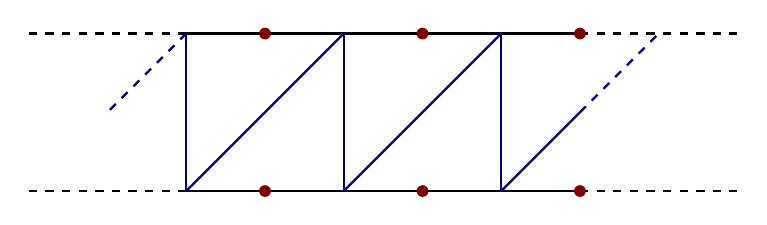
\begin{tikzpicture}
            \draw [thick] (2,2) -- (7,2);
            \draw [thick,dashed] (0,2) -- (2,2);
            \draw [thick, dashed] (7,2) -- (9,2);
            \draw [thick,dashed] (0,0) -- (2,0);
            \draw [thick,dashed] (7,0) -- (9,0);
            \draw [thick] (2,0) -- (7,0);
            \foreach \x in {3,5,7} {
                \node [circle,fill=red!50!black, inner sep=1.5pt] at (\x, 2) {};
                \node [circle,fill=red!50!black,inner sep=1.5pt] at (\x,0) {};
            }
            \draw [thick,blue!50!black] (4,0) -- (4,2);
            \draw [thick,blue!50!black] (4,0) -- (6,2);
            \draw [thick,blue!50!black] (6,2) -- (6,0);
            \draw [thick,blue!50!black] (4,2) -- (2,0);
            \draw [thick,blue!50!black] (6,0) -- (7,1);
            \draw [thick, blue!50!black,dashed] (7,1) -- (8,2);
% ---- 原文行 1140 ----
            \draw [thick, blue!50!black] (2,0) -- (2,2);
            \draw [thick, blue!50!black, dashed] (2,2) -- (1,1);
        \end{tikzpicture}
        \caption{Generating Lagrangians of $\mathcal{W} (\mathbb{C}, e^z+e^{-z})$.}\label{fig:generating-Lag-equiv-P1}
    \end{figure}
    The space $(\mathbb{C},e^z+e^{-z})$ can be pictured as in figure \ref{fig:generating-Lag-equiv-P1}, where the red dots are fibres of $e^z+e^{-z}$ near infinity, and blue lines are Lagrangian submanifolds that are projected diffeomorphically onto $\mathbb{C}^{\ast}$ via the exponential map $z\mapsto e^z$. We claim that these Lagrangian submanifolds generate the wrapped Fukaya category $\mathcal{W} (\mathbb{C},e^z+e^{-z})$.\par
    To prove the claim, first consider the trivial Weinstein sector $X_0\coloneqq(\mathbb{C},z^2) \simeq T^{\ast} [0,1]$, then the Weinstein sector $(\mathbb{C},e^z+e^{-z})$ can be regarded as attaching $\mathbb{Z}$-copies of $1$-handles to the disjoint union \[
        \bigsqcup_{\mathbb{Z}} X_0
    \]in the way depicted in figure \ref{fig:1-handle-attaching-Z}. It's then clear that the wrapped Fukaya category $\mathcal{W} (\mathbb{C},e^z+e^{-z})$ is generated by the union of blue Lagrangians in figure \ref{fig:1-handle-attaching-Z}, as they are generalized cocores to the sector $X_0$ and to the $1$-handles. It's not difficult to check that these Lagrangians are exactly the blue Lagrangians shown in figure \ref{fig:generating-Lag-equiv-P1}.\par
    \begin{figure}[ht]
        \centering
        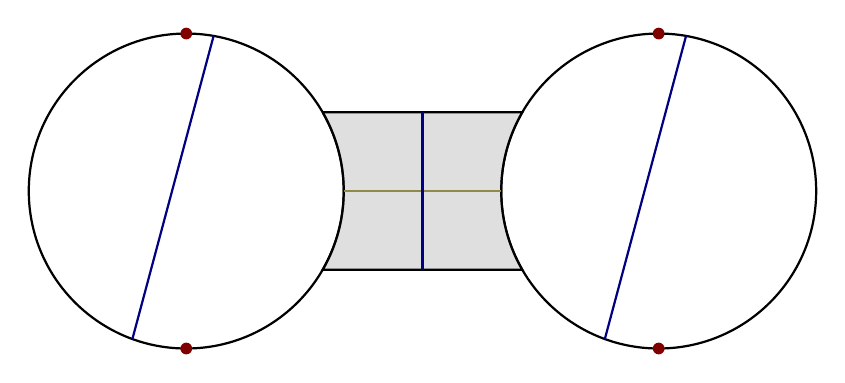
\begin{tikzpicture}
            \begin{scope}
                \draw [thick] (0,0) circle (2);
                \node [circle, fill=red!50!black, inner sep=1.5pt] at (0,2) {};
                \node [circle, fill=red!50!black, inner sep=1.5pt] at (0,-2) {};
            \end{scope}
            \begin{scope}[xshift=6cm]
                \draw [thick] (0,0) circle (2);
                \node [circle, fill=red!50!black, inner sep=1.5pt] at (0,2) {};
% ---- 原文行 1160 ----
                \node [circle, fill=red!50!black, inner sep=1.5pt] at (0,-2) {};
            \end{scope}
            \filldraw[ fill=lightgray, fill opacity=0.5, draw=black, thick ] ({2*cos(30)},{2*sin(30)}) -- ({6+2*cos(150)},{2*sin(150)}) arc [start angle = 150, end angle = 210, radius = 2] -- ({2*cos(-30)},{2*sin(-30)}) arc [start angle = -30, end angle = 30, radius = 2];
            \draw [thick, yellow!50!black] (2,0) -- (4,0);
            \draw [thick, blue!50!black] ({2*cos(250)},{2*sin(250)}) -- ({2*cos(80)},{2*sin(80)});
            \draw [thick,blue!50!black] (3,{-2*sin(30)}) -- (3,{2*sin(30)});
            \draw [thick,blue!50!black] ({6+2*cos(250)},{2*sin(250)}) -- ({6+2*cos(80)},{2*sin(80)});
        \end{tikzpicture}
        \caption{Connecting Two ``Standard Copies'' by a $1$-Handle.}\label{fig:1-handle-attaching-Z}
    \end{figure}
    Before we compute the wrapped Floer cohomology of these Lagrangians, we fix one and label the vertical blue Lagrangians (corresponding to the cocore to the $1$-handle in figure \ref{fig:1-handle-attaching-Z}) in figure \ref{fig:generating-Lag-equiv-P1} by $L_0[k]$, $k\in\mathbb{Z}$, and the slanted Lagrangians (corresponding to the generating Lagrangian of $X_0$ in figure \ref{fig:1-handle-attaching-Z}) in figure \ref{fig:generating-Lag-equiv-P1} by $L_1 [k]$. They correspond under Homological Mirror Symmetry to the objects $\mathcal{O}_{\mathbb{P}^1}[k]$ and $\mathcal{O}_{\mathbb{P}^1} (1) [k]$, where $k$ is the character of the $\mathbb{G}_m$-action.\par
    It's clear from figure \ref{fig:1-handle-attaching-Z} that\[
        CW^{\ast} (L_1[k],L_1[l])=\left\{\begin{array}{ll}
            0,&\text{if}\ l\neq k;\\
            \Bbbk,&\text{if}\ l=k.
        \end{array}\right.\quad\text{and}\quad CW^{\ast} (L_0 [k],L_0[l])=\left\{\begin{array}{ll}
            0,&\text{if}\ l\neq k;\\
            \Bbbk,&\text{if}\ l=k.
        \end{array}\right.
    \]Let's conventionally set $L_1[0]$ to be the Lagrangian in the $1$-handle to the right of $X_0[0]$ where $L_1[0]$ lies in. Under this convention, it is also clear that \[
% ---- 原文行 1180 ----
        CW^{\ast} (L_0[k],L_1 [l])=\left\{\begin{array}{ll}
            0,&\text{if}\ \vert k-l\vert\geq 2;\\ 
            \Bbbk,&\text{otherwise}.
        \end{array}\right.\quad\text{and}\quad CW^{\ast} (L_1[k],L_0[l])=0.
    \]Therefore we have completely compute the wrapped Fukaya category $\mathcal{W} (\mathbb{C}, e^z+e^{-z})$. To summarize, $\mathcal{W} (\mathbb{C},e^z+e^{-z})$ is quasi-equivalent to the category of complexes of perfect modules over path algebras of the infinite quiver \[
        \begin{tikzcd}
            &\dotsb &&L_1[0] &&L_1 [1] &&\dotsb&\\
            \dotsb&&L_0[0]\arrow[ru]\arrow[lu]&&L_0[1]\arrow[ru]\arrow[lu]&&\dotsb\arrow[lu]
        \end{tikzcd}
    \]
\end{exmp}
\begin{exmp}\label{exmp:wrapped-Fukaya-cat-twice-punctured-equivariant}
    As another example, we will construct a $\mathbb{Z}^2$-cover $\mathcal{X}$ of the Weinstein sector $(\mathbb{C}\setminus\{\pm 1\},2/(1-z^2))$. This Weinstein sector can be regarded as the sectorial gluing of two Weinstein sectors $\left(\mathbb{C}^{\ast},z+z^{-1}\right)$ along one of their boundary stops, and its $\mathbb{Z}^2$-cover can be then realized as the gluing of $\mathbb{Z}$-copies of each sector along $\mathbb{Z}^2$-copies of strips, as shown in figure \ref{fig:Z2-cover-twice-punctured-disk}.\par
    \begin{figure}[ht]
        \centering
        \begin{tikzpicture}       
        \begin{scope}[yshift=6cm]
            \draw [thick] (0,0) -- (0,2);
            \draw [thick] (1,0) -- (1,2);
                \foreach \x in {0.2,0.8,1.4}{
% ---- 原文行 1200 ----
                \filldraw [fill=white, draw=black,thick] (1,\x)
            -- (1.2,\x)
            .. controls (1.25,\x)
                       and (1.35,{0.98*\x+0.02*((\x-0.2)/0.2-4.6)})
            .. (1.4,{0.96*\x+0.04*((\x-0.2)/0.2-4.6)})
            -- (3.7,{0.04*\x+0.96*((\x-0.2)/0.2-4.6)})
            .. controls (3.75,{0.02*\x+0.98*((\x-0.2)/0.2-4.6)})
                       and (3.8,{(\x-0.2)/0.2-4.6})
            .. (4,{(\x-0.2)/0.2-4.6}) -- (4,{(\x-0.2)/0.2 -4.2})
            .. controls (3.7,{(\x-0.2)/0.2-4.2}) and (3.6,{((\x-0.2)/0.2-4.2)-0.2*((\x-0.2)/0.2-4.6-\x)/2.5})
            .. (3.5,{((\x-0.2)/0.2-4.2)-0.3*((\x-0.2)/0.2-4.6-\x)/2.5})
            -- (1.5,{\x+0.4+0.3*((\x-0.2)/0.2-4.6-\x)/2.5})
            .. controls (1.4,{\x+0.4+0.2*((\x-0.2)/0.2-4.6-\x)/2.5}) and (1.3,{\x+0.4})
            ..(1.2,{\x+0.4}) -- (1,{\x+0.4}) -- cycle;
            }
            \foreach \x in {0.4,1,1.6} {
                \node [circle,fill=red,inner sep=1.5pt] at (0,\x) {};
                \node [circle,fill=red,inner sep=1.5pt] at (1,\x) {};
            }
        \end{scope}
% ---- 原文行 1220 ----
        \begin{scope}[yshift=3cm]
            \draw [thick] (0,0) -- (0,2);
            \draw [thick] (1,0) -- (1,2);
            \foreach \x in {0.2,0.8,1.4}{
                \filldraw [fill=white, draw=black, thick] (1,\x)
            -- (1.2,\x)
            .. controls (1.25,\x)
                       and (1.35,{0.98*\x+0.02*((\x-0.2)/0.2-2.2)})
            .. (1.4,{0.96*\x+0.04*((\x-0.2)/0.2-2.2)})
            -- (3.7,{0.04*\x+0.96*((\x-0.2)/0.2-2.2)})
            .. controls (3.75,{0.02*\x+0.98*((\x-0.2)/0.2-2.2)})
                       and (3.8,{(\x-0.2)/0.2-2.2})
            .. (4,{(\x-0.2)/0.2-2.2}) -- (4,{(\x-0.2)/0.2 -1.8})
            .. controls (3.7,{(\x-0.2)/0.2-1.8}) and (3.6,{((\x-0.2)/0.2-1.8)-0.2*((\x-0.2)/0.2-2.2-\x)/2.5})
            .. (3.5,{((\x-0.2)/0.2-1.8)-0.3*((\x-0.2)/0.2-2.2-\x)/2.5})
            -- (1.5,{\x+0.4+0.3*((\x-0.2)/0.2-2.2-\x)/2.5})
            .. controls (1.4,{\x+0.4+0.2*((\x-0.2)/0.2-2.2-\x)/2.5}) and (1.3,{\x+0.4})
            ..(1.2,{\x+0.4}) -- (1,{\x+0.4}) -- cycle;
            }
            \foreach \x in {0.4,1,1.6} {
% ---- 原文行 1240 ----
                \node [circle,fill=red,inner sep=1.5pt] at (0,\x) {};
                \node [circle,fill=red,inner sep=1.5pt] at (1,\x) {};
            }
        \end{scope}
        \begin{scope}
            \draw [thick] (0,0) -- (0,2);
            \draw [thick] (1,0) -- (1,2);
            \foreach \x in {0.2,0.8,1.4}{
                \filldraw [fill=white, draw=black,thick] (1,\x)
            -- (1.2,\x)
            .. controls (1.25,\x)
                       and (1.35,{0.98*\x+0.02*((\x-0.2)/0.2+0.2)})
            .. (1.4,{0.96*\x+0.04*((\x-0.2)/0.2+0.2)})
            -- (3.7,{0.04*\x+0.96*((\x-0.2)/0.2+0.2)})
            .. controls (3.75,{0.02*\x+0.98*((\x-0.2)/0.2+0.2)})
                       and (3.8,{(\x-0.2)/0.2+0.2})
            .. (4,{(\x-0.2)/0.2+0.2}) -- (4,{(\x-0.2)/0.2 +0.6})
            .. controls (3.7,{(\x-0.2)/0.2+0.6}) and (3.6,{((\x-0.2)/0.2+0.6)-0.2*((\x-0.2)/0.2+0.2-\x)/2.5})
            .. (3.5,{((\x-0.2)/0.2+0.6)-0.3*((\x-0.2)/0.2+0.2-\x)/2.5})
            -- (1.5,{\x+0.4+0.3*((\x-0.2)/0.2+0.2-\x)/2.5})
% ---- 原文行 1260 ----
            .. controls (1.4,{\x+0.4+0.2*((\x-0.2)/0.2+0.2-\x)/2.5}) and (1.3,{\x+0.4})
            ..(1.2,{\x+0.4}) -- (1,{\x+0.4}) -- cycle;
            }
            \foreach \x in {0.4,1,1.6} {
                \node [circle,fill=red,inner sep=1.5pt] at (0,\x) {};
                \node [circle,fill=red,inner sep=1.5pt] at (1,\x) {};
            }
        \end{scope}
        \begin{scope}[yshift=3cm, xshift=4cm]
            \draw [thick] (0,0) -- (0,2);
            \draw [thick] (1,0) -- (1,2);
            \foreach \x in {0.4,1,1.6} {
                \node [circle,fill=red,inner sep=1.5pt] at (0,\x) {};
                \node [circle,fill=red,inner sep=1.5pt] at (1,\x) {};
            }
        \end{scope}     
        \begin{scope}[xshift=4cm]
            \draw [thick] (0,0) -- (0,2);
            \draw [thick] (1,0) -- (1,2);
            \foreach \x in {0.4,1,1.6} {
% ---- 原文行 1280 ----
                \node [circle,fill=red,inner sep=1.5pt] at (0,\x) {};
                \node [circle,fill=red,inner sep=1.5pt] at (1,\x) {};
            }
        \end{scope}
        \begin{scope}[yshift=6cm,xshift=4cm]
            \draw [thick] (0,0) -- (0,2);
            \draw [thick] (1,0) -- (1,2);
            \foreach \x in {0.4,1,1.6} {
                \node [circle,fill=red,inner sep=1.5pt] at (0,\x) {};
                \node [circle,fill=red,inner sep=1.5pt] at (1,\x) {};
            }
        \end{scope}
        \begin{scope}[yshift=9cm]
            \node at (0.5,1) {$\vdots$};
        \end{scope}
        \begin{scope}[yshift=-3cm]
            \node at (0.5,1) {$\vdots$};
        \end{scope}
        \begin{scope}[yshift=9cm,xshift=4cm]
            \node at (0.5,1) {$\vdots$};
% ---- 原文行 1300 ----
        \end{scope}
